%\documentclass[useAMS, usenatbib,usegraphicx,letter]{mn2e}
%\documentclass[11pt]{article}
\documentclass[reprint,aps,prd,superscriptaddress,showkeys,showpacs]{revtex4-1}
\usepackage{epsfig,amsmath,natbib}

\usepackage{aas_macros}
\usepackage{amssymb}
\usepackage{amsmath}
\usepackage{dsfont}
\usepackage{hyperref}
\usepackage{color}
\usepackage{pbox}
\usepackage{booktabs}

\hypersetup{
	colorlinks=false,
	citecolor=green
}
% \usepackage{graphicx}
% \usepackage{epstopdf}
% \usepackage{natbib}

%%%%%%%%%%%%%%%%%
%Custom commands%
%%%%%%%%%%%%%%%%%

\newcommand{\bb}[1]{\mathbf{#1}}
\newcommand{\bbh}[1]{\mathbf{\hat{#1}}}
\newcommand{\h}[1]{\hat{#1}}
\newcommand{\ttt}[1]{\texttt{#1}}

%%%%%%%%%%%%%%%%%%%%%%%%%%%%%%%%%%%%%%%%%%%%%%

\begin{document}

\title{Mocking the Weak Lensing universe: the LensTools computing package}

\author{Andrea Petri}
\email{apetri@phys.columbia.edu}
\affiliation{Department of Physics, Columbia University, New York, NY 10027, USA}
\affiliation{Physics Department, Brookhaven National Laboratory, Upton, NY 11973, USA}

\date{\today}

\label{firstpage}

\begin{abstract}
We present a newly developed software package which implements a wide range of routines frequently used in Weak Gravitational Lensing (WL). With the continuously increasing size of the WL scientific community we feel that easy to use APIs for common calculations are a necessity to ensure efficiency and coordination across different working groups. Coupled with existing open source codes, such as \ttt{CAMB}\citep{CAMB} and \ttt{GADGET2}\citep{Gadget2}, \ttt{LensTools} brings together a fully functional cosmic shear simulation pipeline which, coupled with a variety of WL feature measurement tools and parameter sampling routines, provides easy access to the numerics for theoretical studies of WL as well as for experiment forecasts. Being implemented in \ttt{python}\citep{python}, \ttt{LensTools} takes full advantage of a range of state--of--the art techniques developed by the large and growing open--source software community.    
    
\end{abstract}


\keywords{Weak Gravitational Lensing --- Simulations}
\pacs{98.80.-k, 95.36.+x, 95.30.Sf, 98.62.Sb}

\maketitle


%%%%%%%%%%%%%%%%%%%%%%%%%% INTRO %%%%%%%%%%%%%%%%%%%%%%%%%%%%%%%%%%%%%%%%%%%%%%%%%%%%%%%%

\section{Introduction}
%
Cosmology is entering a new, data driven era. After the Cosmic Microwave Background (CMB) \citep{WMAP,PlanckXVI2013} provided strong experimental evidences of cosmological theories, a variety of different probes have been proposed to unveil the secret of the cosmos. Weak Gravitational Lensing uses the correlation between image distortions of background sources by Large Scale Structure (LSS) to infer cosmological parameters \citep{WLprimer}. Because WL probes are sensitive to the late universe, where the density fluctuations are in the non--linear regime, the cosmological information might not be all contained in quadratic features such as two--point correlation functions. In the theoretical study of more complicated WL features (see for example \citep{3pcf1,bispectrum1,moments1,peaks1} for a non comprehensive list), simulation pipelines play a vital role as in general these features cannot be predicted analitically from the cosmological parameters. In this work we present a flexible, customizable and easy to deploy WL simulation pipeline that bridegs the gap between simulations of shear fields, feature measurement from simulated images and cosmological parameter estimation. The paper is organized as follows: first we give an overview of the code structure, highlight the core routines and present the benchmarks and complexity of the expensive computing steps. We complement the work with some illustrative examples on how to use \ttt{LensTools} for some of the former tasks. We finally discuss the future prospects of the software development.     

%%%%%%%%%%%%%%%%%%% CODE %%%%%%%%%%%%%%%%%%%%%%%%%%%%%%%%%%%%%%%

\section{Code} 

\subsection{Shear field simulations}

\begin{figure*}
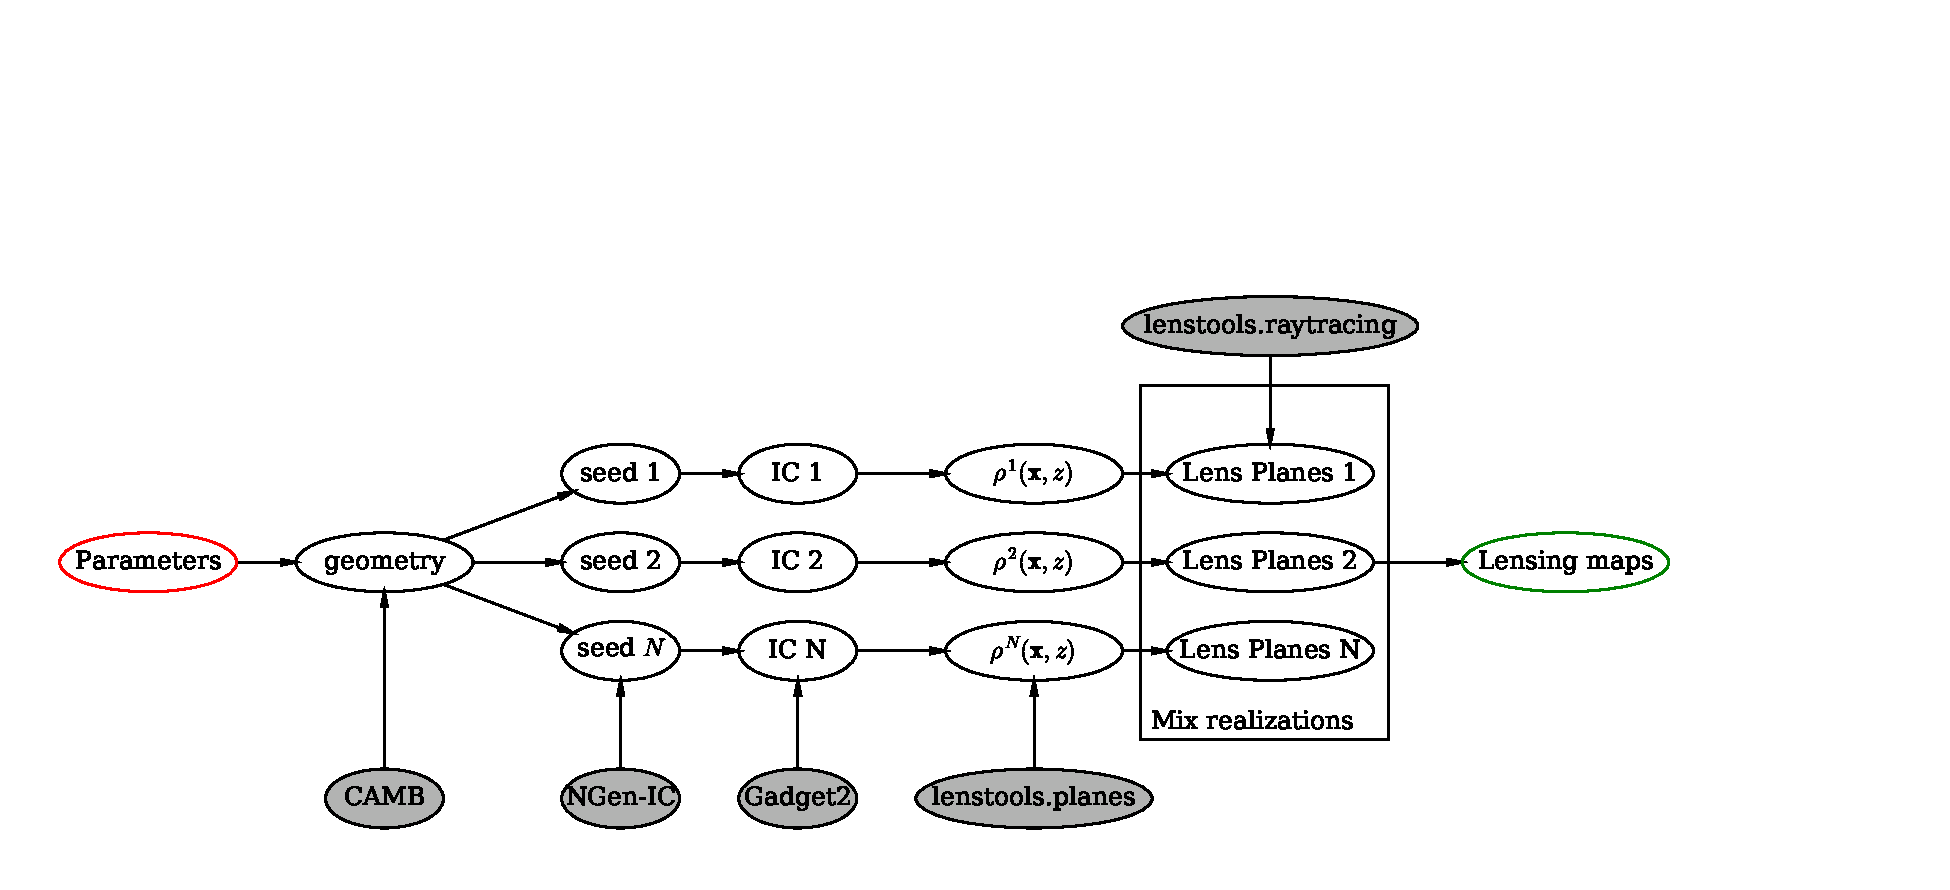
\includegraphics[scale=0.6]{Figures/flow.eps}
\end{figure*}

\begin{table*}
\begin{tabular}{l|c|c|c}
\toprule
{Step} &            Complexity &            Test case &           Runtime \\ \hline \hline
\midrule
\multicolumn{4}{c}{\textbf{Lens generation}} \\ \hline
Snapshot input & $O(N_p/N_t)$  & $N_p=512^3$, $N_t=16$  &  \\
Gridding        & $O(N_p/N_t)$   & $N_p=512^3$, $N_t=16$  &  \\
MPI Communication  & $O(L_p\log{N_t})$   & $N_t=16$, $L_p=4096^2$  &   \\
Poisson solver           & $O(L_p\log{L_p})$ & $L_p=4096^2$  &      \\
Lens output           & $O(L_p)$ & $L_p=4096^2$   &   \\ \hline \hline

\multicolumn{4}{c}{\textbf{Ray tracing}} \\ \hline
Lens input &  $O(L_p)$ & $L_p=4096^2$ &  \\
Random lens shift &  $O(L_p)$ & $L_p=4096^2$ &  \\
Deflection calculation        &  $O(M_p)$ & $M_p=2048^2$   &  \\
Shear tensor product               &  $O(M_p)$ & $M_p=2048^2$   &   \\ \hline \hline

\bottomrule
\end{tabular}
\caption{Ray tracing benchmarks}
\label{benchmarktable}
\end{table*}



\subsection{Weak lensing features}

\subsection{Parameter estimation}

%%%%%%%%%%%%%%%%%%% EXAMPLES %%%%%%%%%%%%%%%%%%%%%%%%%%%%%%%%%%%%%%%

\section{Examples}

%%%%%%%%%%%%%%%%%% FUTURE %%%%%%%%%%%%%%%%%%%%%%%%%%%%%%%%%%%%%

\section{Future developments}

%%%%%%%%%%%%%%%%%% CONCLUSION %%%%%%%%%%%%%%%%%%%%%%%%%%%%%%%%%%%%%

\section{Conclusion}

%%%%%%%%%%%%%%%%%%%%%%%%%% ACKNOWLEDGMENTS %%%%%%%%%%%%%%%%%%%%%%%%%%%%%%%%%%%%%%%%%%%%%%%%%%%%%%
 

\section*{Acknowledgements}


\bibliography{ref}
\label{lastpage}
\end{document}
